\section{K-means codebook}
\label{sec:intro}

We implemented the classification process following the visual codebook pipeline provided in the instruction. First, we extracted 100K SIFT feature descriptors from the training data and applied K-means clustering to construct a visual vocabulary.

%-------------------------------------------------------------------------
\subsection{Vocabulary size of K-means clustering}
Theoretically, a small visual vocabulary size $K$ increases the risk of underfitting but offers better time-wise efficiency. Conversely, a large $K$ poses a higher risk of overfitting and results in lower efficiency. Theoretically, the time complexity of K-means clustering and vector quantization is proportional to the value of $K$, and our result \cref{fig:q1-fig1} align with it.

\begin{figure}[htbp]
	\centering
	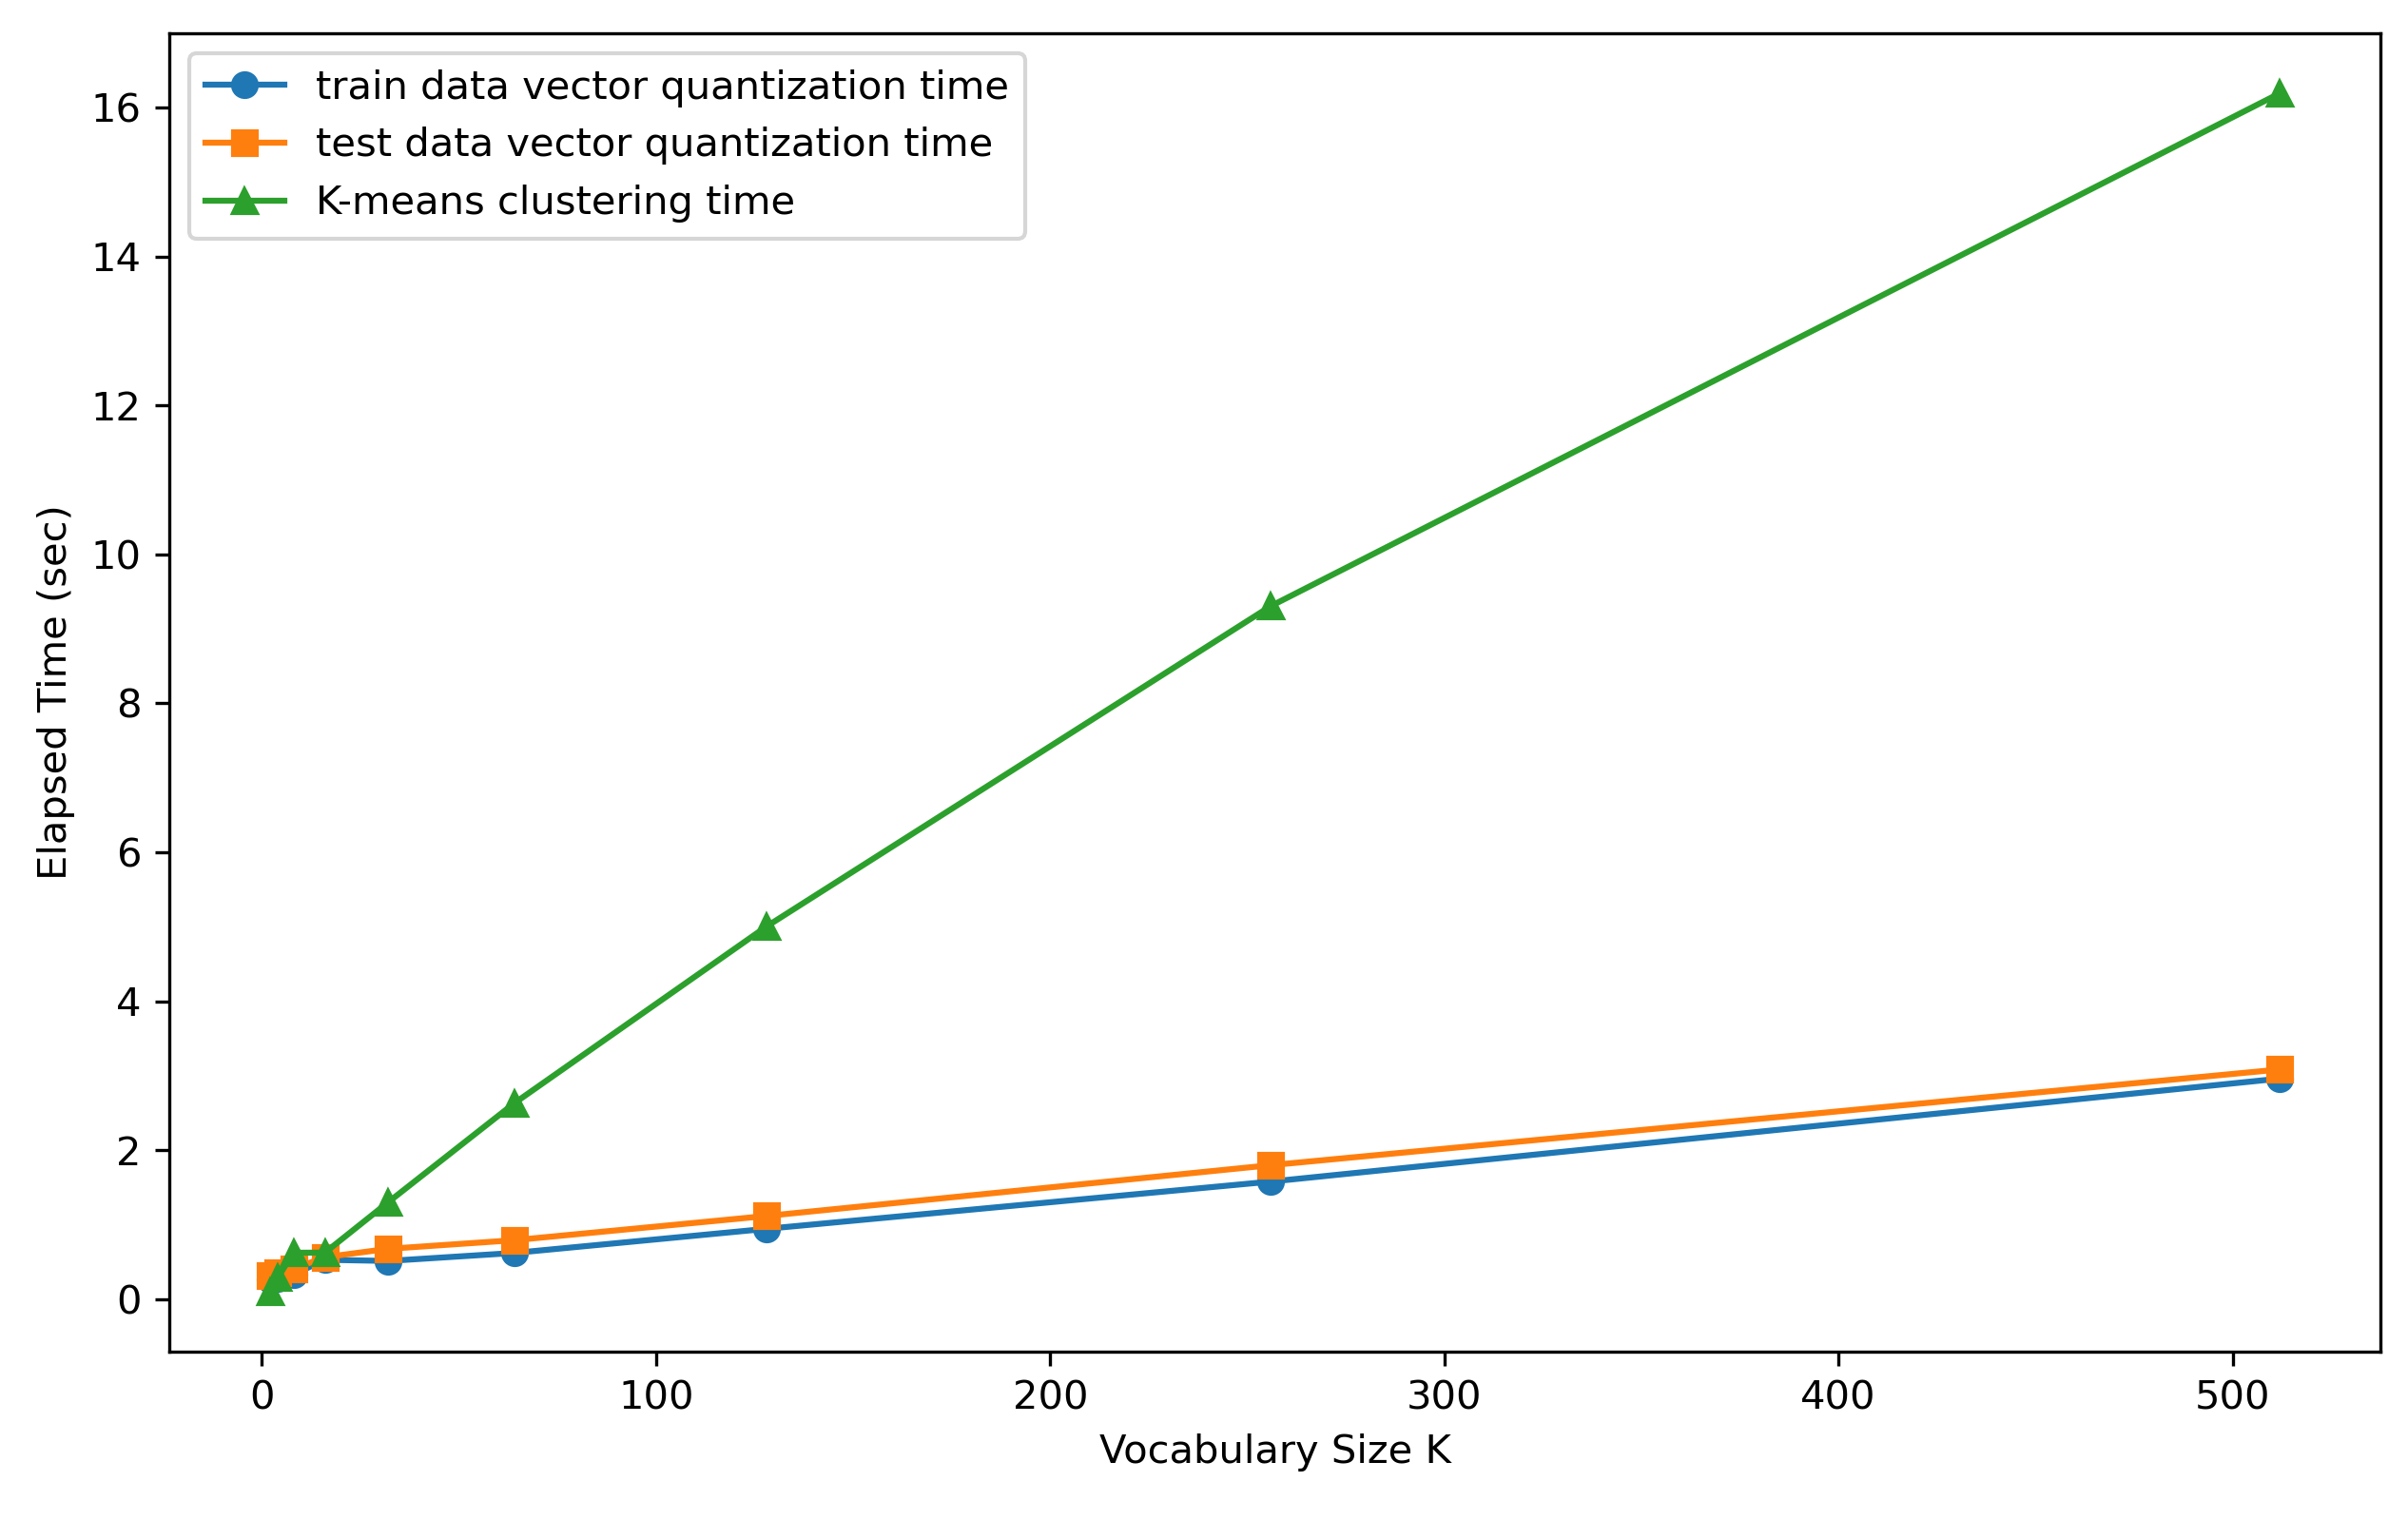
\includegraphics[width=0.4\linewidth]{image/q1-fig1.png}
	\caption{K-means visual vocabulary: training and quantization time according to the value of $k$}
	\label{fig:q1-fig1}
\end{figure}

\subsection{Vector quantisation process}
\label{subsec:Q1_2}
To quantize images, SIFT feature descriptors from each image were mapped to their nearest vocabulary clusters, generating a histogram vector based on the cluster frequencies. This reduced each image's dimension to the visual vocabulary size, $K$. \cref{fig:q1-fig2} visualizes these histograms for different word sizes, illustrating underfitting and overfitting issues related to $K$. For $K=4$, the histogram cosine similarity between the 2nd and 3rd images is higher than between the 1st and 2nd images. However, as $K$ increases, similarity between the 1st and 2nd images (same class) improves. Furthermore, excessively large $K$ reduces inner-class similarity, risking overfitting in classification. Additional histogram samples and cosine similarity measurements are detailed in \cref{subsec:Q1_histograms} and \cref{subsec:Q1_cossim}.
 
 \begin{figure}
 	\centering
 	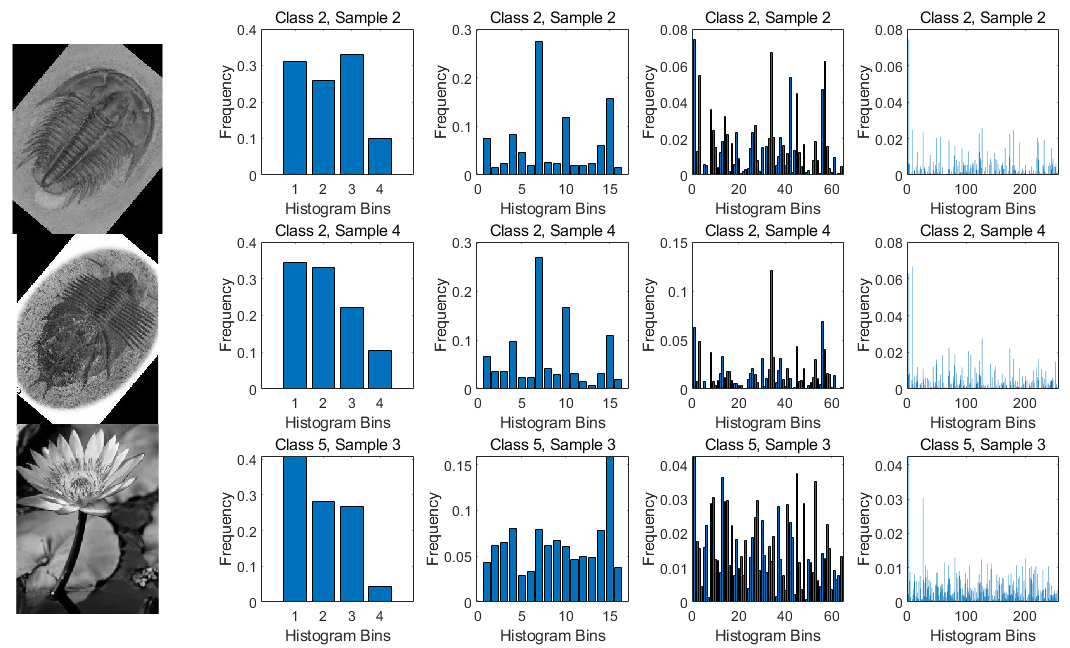
\includegraphics[width=0.4\linewidth]{image/q1-fig2.png}
 	\caption{K-means visual vocabulary: training and quantization time according to the value of $k$}
 	\label{fig:q1-fig2}
 \end{figure}
 